\input{../header.tex}
\usepackage{etoolbox}
\usepackage{placeins}
\usepackage{tikz}
\usepackage{fontawesome6}
\usepackage[T1]{fontenc}
\usetikzlibrary{arrows.meta}

\usetikzlibrary{decorations.pathreplacing}
\usepackage[dvipsnames]{xcolor}
\usetikzlibrary{trees}

% Define colors
\definecolor{javared}{rgb}{0.6,0,0}
\definecolor{javagreen}{rgb}{0.25,0.5,0.35}
\definecolor{javapurple}{rgb}{0.5,0,0.35}
\definecolor{javadocblue}{rgb}{0.25,0.35,0.75}
\definecolor{pythonblue}{rgb}{0,0,0.6}
\definecolor{pythongreen}{rgb}{0,0.5,0}
\definecolor{pythonred}{rgb}{0.6,0,0}
\definecolor{pythongray}{rgb}{0.5,0.5,0.5}

% Java listing style
\lstdefinestyle{javastyle}{
    language=Java,
    basicstyle=\ttfamily\small,
    keywordstyle=\color{javapurple}\bfseries,
    stringstyle=\color{javared},
    commentstyle=\color{javagreen}\itshape,
    morecomment=[s][\color{javadocblue}]{/**}{*/},
    numbers=left,
    numberstyle=\tiny\color{gray},
    numbersep=8pt,
    tabsize=4,
    showspaces=false,
    showstringspaces=false,
    breaklines=true,
    frame=single,
    rulecolor=\color{black},
    backgroundcolor=\color{white},
    captionpos=b,
    xleftmargin=2em,
    framexleftmargin=1.5em
}

% Python listing style
\lstdefinestyle{pythonstyle}{
    language=Python,
    basicstyle=\ttfamily\small,
    keywordstyle=\color{pythonblue}\bfseries,
    stringstyle=\color{pythonred},
    commentstyle=\color{pythongray}\itshape,
    numbers=left,
    numberstyle=\tiny\color{gray},
    numbersep=8pt,
    tabsize=4,
    showspaces=false,
    showstringspaces=false,
    breaklines=true,
    frame=single,
    rulecolor=\color{black},
    backgroundcolor=\color{white},
    captionpos=b,
    xleftmargin=2em,
    framexleftmargin=1.5em,
    morekeywords={self,True,False,None,as,with}
}


\newcommand{\mcqlist}[1]{%
  \begin{enumerate}[label=(\Alph*), itemsep=0.5em]
    \def\do##1{\item ##1}
    \docsvlist{#1}
  \end{enumerate}
}

\usepackage{listings}
\usepackage{array}
\lstset{upquote=true,basicstyle=\fontencoding{T1}\selectfont\ttfamily}

\newcolumntype{C}[1]{>{\centering\let\newline\\\arraybackslash\hspace{0pt}}m{#1}}

\begin{document}

    % Change the following values to true to show the solutions or/and the hints
    \ShowSolutiontrue
    \ShowConseiltrue
    \ShowWarningtrue
    \titre
    \cours{Banque des questions}

\begin{Exercice}[10 minutes]\textbf{Sean}

Dans cette exercice nous aimerions que le processeur calcule et enregistre le produit de 3 fois $10_{10}$ ($00001010_2$) dans le registre 11. Le program counter (PC) commence à \textbf{00000100} et les registres sont initialisés comme suit:

\begin{center}
\begin{tabular}{|c|l|}
\hline
\textbf{Registre} & \textbf{Valeur} \\
\hline
00 & 00001010 \\
01 & 00000000 \\
10 & 00000000 \\
11 & 00000000 \\
\hline
\end{tabular}
\end{center}

Les opérations disponibles sont:

\begin{center}
\begin{tabular}{|c|c|}
\hline
\textbf{Numéro} & \textbf{Instruction} \\
\hline
00 & MOV \\
01 & XOR \\
10 & ADD \\
11 & SUB \\
\hline
\end{tabular}
\end{center}

\bigskip % Creates vertical space, equivalent to Typst's \ \

% --- Part a ---
\noindent % Prevents indentation
\textbf{a.} Complétez le tableau ci-dessous avec les instructions en binaire nécessaires pour effectuer cette tâche.

\begin{center}
\begin{tabular}{|l|l|}
\hline
\textbf{Adresse} & \textbf{Valeur} \\
\hline
00000100 & \\
00000101 & \\
\hline
\end{tabular}
\end{center}

\bigskip

% --- Part b ---
\noindent % Prevents indentation
\textbf{b.} Donnez le contenu des registres après l'éxécution de la première instruction et après l'éxécution de la deuxième instruction.

\begin{center}
\begin{tabular}{|c|l|l|}
\hline
\textbf{Registre} & \textbf{Après 1ère instruction} & \textbf{Après 2ème instruction} \\
\hline
00 & & \\
01 & & \\
10 & & \\
11 & & \\
\hline
\end{tabular}
\end{center}
\end{Exercice}

\begin{Exercice}[15 minutes]\textbf{Sean}
Quel est le résultat de la soustraction hexadécimale suivante: 694F - 5A3C ?
\end{Exercice}


\begin{Exercice}[10 minutes]\textbf{Aurore}
Selon le modèle de Von Neumann, partant d'un program counter valant 101010 et d'une mémoire contenant les instructions suivantes:
\begin{table}[h]
\centering
\begin{tabular}{|c|c|}
\hline
\textbf{Adresse} & \textbf{Instruction} \\
\hline
101001 & 01000111 \\
101010 & 01111000 \\
101011 & 10001101 \\
101100 & 10010110 \\
\hline
\end{tabular}
\end{table}

À quelle adresse le résultat de la prochaine opération va-t-il être stocké?

\mcqlist{00, 01, 10, 11}

\end{Exercice}

\begin{Exercice}[10 minutes]\textbf{Aurore} Quel est le résultat de l'opération suivante : $395_{16}$ + $1011101_{2}$?
\mcqlist{$1010_{10}$, $3E2_{16}$, $0011 1110 0010_2$, $1010_2$}

\end{Exercice}

\begin{Exercice}[10 minutes]\textbf{Maxim} Quelle est la valeur en base 10 de l’opération suivante : $128_9$ - $245_6$?
\mcqlist{9,6,0,3}
\end{Exercice}

\begin{Exercice}[10 minutes]\textbf{Maxim}
Convertir le nombre $127_{10}$ en base 8.
\mcqlist{87,177,71,180}
\end{Exercice}

\begin{Exercice}[10 minutes]\textbf{Léa}
Quel est le résultat de l'opération suivante $67_8$ + $110111_2$ en base 10? 
\mcqlist{110, 78, 122, 106}
\end{Exercice}

\begin{Exercice}[10 minutes]\textbf{Léa}
En suivant le modèle de von Neuman, l'instruction register (IR) a une valeur de 11000111, les registres contiennent les valeurs suivantes:
\begin{table}[h!]
\centering
\begin{tabular}{|c|c|}
\hline
\textbf{Registre} & \textbf{Valeur} \\ \hline
00 & 00000000 \\ 
01 & 00000101 \\ 
10 & 00000110 \\ 
11 & 00000010 \\ \hline
\end{tabular}
\end{table}

\begin{center}
\begin{tabular}{|c|c|}
\hline
\textbf{Numéro} & \textbf{Valeur} \\ \hline
00 & MOV \\ 
01 & XOR \\ 
10 & ADD \\ 
11 & SUB \\ \hline
\end{tabular}
\end{center}
Quelle est la valeur du résultat de l'opération?
\mcqlist{$111_2$, $1011_2$, $011_2$, $0001_2$}
\end{Exercice}

\begin{Exercice}[10 minutes]\textbf{Léa}
Quelle est la valeur du résultat de l'opération?
\mcqlist{$111_2$, $1011_2$, $011_2$, $0001_2$}
\end{Exercice}

\begin{Exercice}[10 minutes]\textbf{Reda}
Que représentent les deux premiers bits de l'instruction register? (exemple: 11001001)?
\mcqlist{L'adresse du registre dans lequel il faudra mettre le résultat,
L'identificateur de l'opération à exécuter,
L'adresse du registre dans lequel est contenue la valeur sur laquelle faire l'opération,
Ils n'ont aucune signification}
\end{Exercice}

\begin{Exercice}[10 minutes]\textbf{Reda}
Quel est le résultat de la soustraction $11011001_2$ - $00110110_2$ en base 10?

\end{Exercice}

\begin{Exercice}[10 minutes]\textbf{Amina}
Quel est le résultat de l'opération suivante : $1011010_2$ - $1000111_2$?
\mcqlist{$0001111_2$, $0010011_2$, $0100011_2$, $0010101_2$}
\end{Exercice}


\begin{Exercice}[10 minutes]\textbf{Amina}
Quel est le résultat en base 10 de l'opération suivante : $47_{10}$ + $DEF_{16}$ ?
\mcqlist{3614, 3478, 3589, 3641}
\end{Exercice}

\begin{Exercice}[10 minutes]\textbf{Maxim}
Quel est l'avantage principal d'un langage compilé ?
\mcqlist{Plus facile à corriger, Exécution plus rapide, Plus simple à écrire que les autres langages, Indépendant du système d’exploitation}
\end{Exercice}

\begin{Exercice}[10 minutes]\textbf{Maxim}
    Quelle est la différence entre un compilateur et un interpréteur ?
    \mcqlist{Le compilateur traduit le code au moment de l’exécution, l’interpréteur avant l’exécution,
    Le compilateur traduit le code avant l’exécution, l’interpréteur au moment de l’exécution,
    Les deux font exactement la même chose,
    Le compilateur n’est utilisé que pour les systèmes Unix}
\end{Exercice}

\begin{Exercice}[10 minutes]\textbf{Léa}

Voici la visualisation de vos dossiers (exemple: Dans le dossier Cours il y a un dossier Cours\_1):

\begin{figure}[h!]
\begin{tikzpicture}[scale=1.6,
    every node/.style = {draw=black, thick, anchor=west},
    selected/.style = {draw=OliveGreen, fill=green!30},
    file/.style = {draw=blue, fill=cyan!30},
    optional/.style = {dashed, fill=gray!50},
    grow via three points={one child at (0.5,-0.7) and two children at (0.5,-0.7) and (0.5,-1.4)},
    edge from parent path={(\tikzparentnode.south) |- (\tikzchildnode.west)}
]
\node [selected] {\faFolder[regular] /User}
child { 
    node [selected] {\faFolder[regular] /Cours}
    child { 
        node [selected] {\faFolder[regular] /Cours\_1}
        child { 
            node [file] {\faFile[regular] Slides\_1.pdf}
        }
    }
}
child [missing] {}
child [missing] {}
child { 
    node [selected] {\faFolder[regular] /TPs}
    child { 
        node [selected] {\faFolder[regular] /Solutions}
    }
    child { 
        node [file] {\faFile[regular] tp1.py}
    }
    child { 
        node [file] {\faFile[regular] tp1.java}
    }
}
child [missing] {}
child [missing] {}
child [missing] {}
child { 
    node [selected] {\faFolder[regular] /Documents}
}
child { 
    node [selected] {\faFolder[regular] /Photos}
};
\end{tikzpicture}
\end{figure}
\FloatBarrier

Vous ouvrez un terminal et vous êtes dans le dossier Tps, qu'est ce qui va être affiché dans le terminal si vous tapez ls (on écrit tout à la même ligne par souci de concision):

\mcqlist{Solutions tp1.py tp1.java, TPs Solutions tp1.py tp1.java, Cours Cours\_1 Slides\_1 TPs Solutions tp1.py tp1.py Photos Documents, tp1.py tp1.java}
\end{Exercice}

\begin{Exercice}[10 minutes]\textbf{Léa}
Vous êtes toujours dans le dossier Tps et vous voulez aller dans le dossier Solutions, quelle commande tapez vous dans le terminal?
\mcqlist{rm Solutions,mv Solutions, cd Solutions, mkdir Solutions}
\end{Exercice}

\begin{Exercice}[10 minutes]\textbf{Sean}


Vous vous trouvez dans un dossier qui contient deux sous-dossiers : \faFolder[regular] \textcolor{blue}{python} et \faFolder[regular] \textcolor{blue}{java}.
\begin{itemize}
    \item[$\bullet$] Le dossier \textcolor{blue}{python} contient un unique fichier nommé \textcolor{green}{hello.py}.
    \item[$\bullet$] Le dossier \textcolor{blue}{java} contient un unique fichier nommé \textcolor{green}{hi.java}.
\end{itemize}

\textbf{(a)} Quelle(s) commande(s) devez-vous taper dans le terminal, ouvert depuis le dossier \textbf{parent} de python, pour exécuter le programme \textit{hello.py} ? \\ 

\textbf{(b)} Après avoir exécuté les commandes de la question (a), quelles commandes faut-il saisir pour compiler puis exécuter le programme \textit{hi.java} situé dans le dossier \textit{java} ? \\ 

\textbf{(c)} Après avoir exécuté le programme \textit{hi.java}, si vous vous placez dans le dossier \textit{java} et que vous tapez la commande \textbf{ls}, quelle sera la sortie affichée dans le terminal ?

% \vspace{1em}
% \noindent\rule{\textwidth}{0.4pt}

% \subsection{Solution}

% \textbf{(a)}

% \begin{lstlisting}[language=bash]
% cd python
% python hello.py
% \end{lstlisting}

% Alternative en une seule commande :

% \begin{lstlisting}[language=bash]
% python python/hello.py
% \end{lstlisting}

% \noindent{\color{Maroon}\rule{4cm}{2pt}}

% \textbf{(b)}

% \begin{lstlisting}[language=bash]
% cd ..
% cd java
% javac hi.java
% java hi
% \end{lstlisting}

% Alternative si vous êtes toujours dans le dossier parent de python :

% \begin{lstlisting}[language=bash]
% cd java
% javac hi.java
% java hi
% \end{lstlisting}

% \noindent{\color{Maroon}\rule{4cm}{2pt}}

% \textbf{(c)}

% La sortie affichée sera :

% \begin{lstlisting}
% hi.java
% hi.class
% \end{lstlisting}

\end{Exercice}
\newpage 
\begin{Exercice}[10 minutes]\textbf{Amina}
La commande pwd sous Linux/MacOS permet de:
\mcqlist{Afficher le chemin absolu du répertoire courant, Supprimer le répertoire courant, Créer un nouveau fichier, Afficher la liste des fichiers dans le répertoire courant.}
\end{Exercice}

\begin{Exercice}[10 minutes]\textbf{Amina}
Parmi ces commandes Linux/MacOS, laquelle permet de créer un nouveau répertoire ?
\mcqlist{ls, cd, mkdir, pwd}

\end{Exercice}

\begin{Exercice}[10 minutes]\textbf{Aurore}
Voici la ligne de commande d'un terminal sur une machine MacOS/Linux (à gauche) et Windows (à droite).

\begin{figure}[h!]
    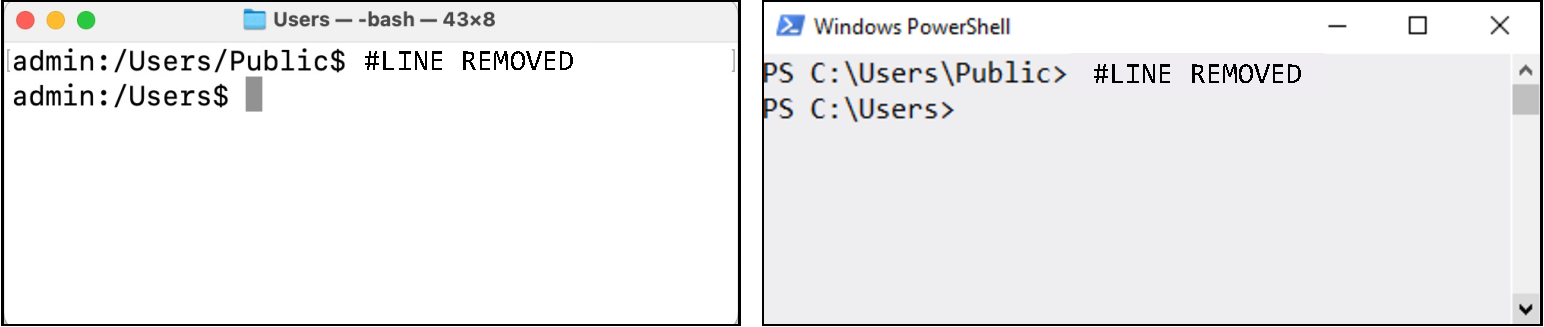
\includegraphics[width = \textwidth]{bashq21.pdf}
\end{figure}

Quelle commande a été passée (\#LINE REMOVED)?

\mcqlist{dir, cd Users, cd .., ls}
\end{Exercice}

\begin{Exercice}[10 minutes]\textbf{Aurore}
Laquelle des affirmations suivantes est fausse?
\mcqlist{Un langage compilé est traduit ligne par ligne au moment de l'exécution, En java, l'étape de compilation et d'interprétation sont séparées, Un langage interprété est plus lent à exécuter, Les langages python et java nécessitent les deux une traduction en bytecode, Toutes les affirmations sont correctes}
\end{Exercice}

\begin{Exercice}[10 minutes]\textbf{Maxim}
En Java, que signifie le mot-clé final appliqué à une variable?
\mcqlist{La variable ne peut pas être utilisée dans une boucle,
La variable est constante et ne peut pas changer de valeur, 
 La variable est automatiquement initialisée à zéro, 
 La variable est globale}

\end{Exercice}

\begin{Exercice}[10 minutes]\textbf{Maxim}
Si on exécute le code suivant:

\begin{lstlisting}[style=pythonstyle]
x = 7 
if x % 2 == 0: 
   print("pair") 
else: 
   print("impair") 
\end{lstlisting}
Que sera affiché?

\mcqlist{impair, pair, 7, Aucun affichage}
\end{Exercice}

\begin{Exercice}[10 minutes]\textbf{Léa}
Qu'affiche le code suivant écrit en Java?

\begin{lstlisting}[style=javastyle]
int numero_jour = 5;
switch (numero_jour) {
    case 1:                
        System.out.println("Lundi");
        break;
    case 2:
        System.out.println("Mardi");
        break;
    case 3:
         System.out.println("Mercredi");
         break;
     case 4:
          System.out.println("Jeudi");
          break;            
     case 5:                
          System.out.println("Vendredi");
     case 6:                
          System.out.println("Samedi");
          break;            
     case 7:                
          System.out.println("Dimanche");
          break;            
     default:                
           System.out.println("Ce n'est pas un jour valide !");
\end{lstlisting}

\mcqlist{Vendredi, Vendredi Samedi Dimanche, Ce n'est pas un jour valide, Vendredi Samedi}
\end{Exercice}

\begin{Exercice}[10 minutes]\textbf{Léa}
Qu'affiche le code suivant écrit en Python?
\begin{lstlisting}[style=pythonstyle]
a = False
b = True
c = False

if (a or b) and (a or not c):
    print("output 1")
elif (a or not b) and (a or c):
    print("output 2")
if (a or not b) and (a or not c):
    print("output 3")
else:
    print("output 4")
\end{lstlisting}
\mcqlist{output 1, output 1 output 4, output 4, output 1 output 3}
\end{Exercice}

\begin{Exercice}[10 minutes]\textbf{Léa}
Ecrivez le complément à 2 de $21_{10}$ sur 8 bits:
\mcqlist{1110 1011, 1110 1010, 0001 0101, 0001 0100}
\end{Exercice}


\end{document}